\documentclass[a4paper, 12pt, onecolumn, oneside]{scrartcl}

\usepackage[utf8]{inputenc}
\usepackage{amsmath}
\usepackage{amssymb}
\usepackage{graphicx}
\usepackage[hidelinks]{hyperref}
\usepackage{float}
\usepackage{enumitem}



\title{%
  Resumos de AS \\
  \large Teste Teorico}

\author{Tiago Almeida}
\date{\today}

\begin{document}

\maketitle

\tableofcontents

\section{Introdução}
Escrever um pequeno overview da matéria que sai para o teste teórico 2
e o que esperar encontrar neste documento

\section{Diagramas UML}

\subsection{Activity Diagram}
\subsection{Use Case Diagram}
\subsection{Class Diagram}
\subsection{Sequence Diagram}
\subsection{State machine Diagram}
\subsection{Package Diagram}
\subsection{Component Diagram}
\subsection{Deployment Diagram}

\section{SDLC}

\textbf{SDLC} (System Development Life Cycle), consiste em 4 fases fundamentais:
\begin{enumerate}
  \item Planeamento
  \begin{itemize}
    \item Fase onde se discute o motivo da existencia do sistema e como construí-lo;
    \item O valor do sistema para a organização é identificado
  \end{itemize}  
  \item Análise (Investigação)
  \begin{itemize}
    \item Fase onde se discute sobre quem irá utilizar o sistema, o que o sistema deve fazer e onde e como será utilizado
    \item Comunicação com os stakeholders para identificar as necessidades e propor soluções.
  \end{itemize}  
  \item Desenho (projeto Técnico)
  \begin{itemize}
    \item Fase onde se decido como o sistema irá ser construido, seja em termos de hardware, software, infraestrutura de rede,
    interface, formulários e relatórios de utilizador, programas especificos, bases de dados e ficheiros que serão necessários.
  \end{itemize}  
  \item Implementação
  \begin{itemize}
    \item Fase onde o sistema é construido
  \end{itemize}  
\end{enumerate}
\textbf{Mnemónica: PADI.}\\
\textbf{NOTA:} Existem passos para cada fase que eu não inclui aqui. Se vier a ser importante, voltar ao slide
`AS-TP05b Processos de software.pdf' (páginas 5 a 8) e adicionar. 

\section{Processos de software}
O SDLC é concretizado usando um \textbf{processo de software} sistemático\\
Um processo de software é um guião para as atividades e tarefas que são necessárias para construir software de qualidade\\
Existem duas metodologias que se podem seguir ao criar software:
\begin{itemize}
  \item Linear/estruturada
  \begin{itemize}
    \item Waterfall
  \end{itemize}
  \item Evolutiva
  \begin{itemize}
    \item Prototyping
    \item Spiral model
    \item Métodos ageis
  \end{itemize}
\end{itemize}
Na primeira metodologia, o metodo \textbf{Linear/estruturado}, todas as atividades a serem realizadas são planeadas em avanço 
e o progresso feito é medido tendo em conta o plano já feito.
\\O exemplo clássico da metodologia Linear/estruturada é modelo \textit{Waterfall}\\ 
\begin{figure}[H]
  \centering
  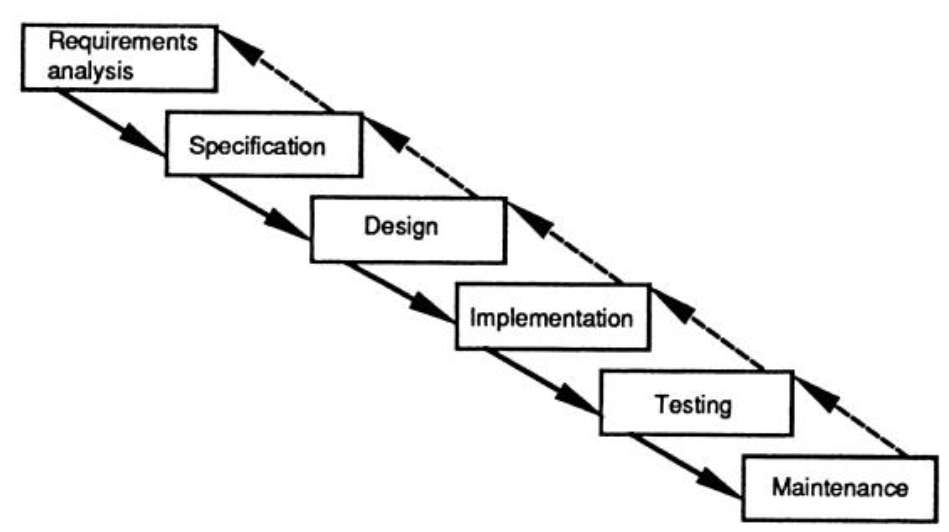
\includegraphics[width=1\textwidth]{waterfall-model.png}
  \caption{Modelo Waterfall}\label{fig1}
\end{figure}
\textbf{Vantagens do modelo Waterfall:}
\begin{itemize}
  \item Facil de planear: Uma agenda pode ser feita com deadlines para cada fase criada.
  \item Facil de  gerenciar: Cada fase tem um processo especifico
  \item Cada fase é feita uma de cada vez, e apenas se avança para a proxima quando se acabar a anterior
  \item Modelo funciona bem quando os requerimentos são simples, estáveis e bem entendidos por quem está a trabalhar\\
\end{itemize}
\textbf{Desvantagens do modelo Waterfall:}
\begin{itemize}
  \item Não é flexivel: Dificil de se adaptar caso acha alguma mudança
  \item Para projetos de longo prazo, o modelo criado no inicio pode ficar desatualizado e não ser mais ideal
  \item Projetos reais raramente conseguem seguir um modelo 100\% sem ter de fazer mudanças
  \item Uma vez que uma versão que trabalhe só é feita no final, o cliente vai ter de esperar até o final do projeto para ver resultados 
  \item O custo de corrigir um erro vai crescendo conforme o projeto avança\\
\end{itemize}
Na segunda metodologia, o metodo \textbf{Evolutivo}, o planeamento é feito de forma incrementativo ao longo do projeto de forma
a ser possivel a adaptação ás necessidades dos clientes.
\\Existem alguns modelos da metodologia Evolutiva apresentada:
\begin{enumerate}
  \item \textbf{Prototyping}
  \begin{itemize}
    \item Consiste em criar um prototipo desde o inicio que os stakeholders devem concordar que serve para definir os requerimentos.
    \item O prototipo é descartado e o sistema real é começado a ser criado com olho na qualidade. 
  \end{itemize}
  \item \textbf{Spiral Model}
  \begin{itemize}
    \item Neste modelo, o projeto passa pelas diferentes fases da evolução repetidas vezes, incluindo a fase de \textit{Deployment}.
    \item Nas iterações iniciais, o projeto liberado ao publico pode ser só um modelo ou protótipo. Nas iterações mais avançadas as versão liberadas 
    vão ficando cada vez mais completas.
    \begin{figure}[H]
      \centering
      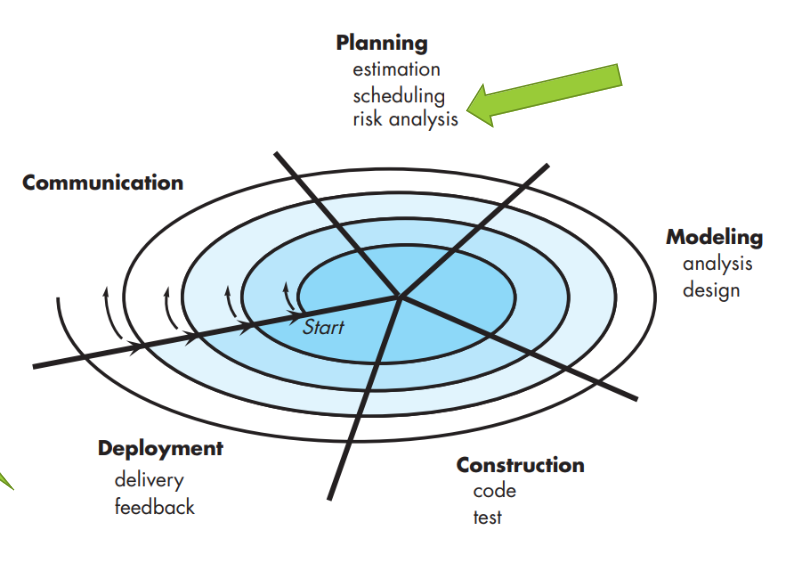
\includegraphics[width=1\textwidth]{modelo-modo-espiral.png}
      \caption{Modelo Waterfall}\label{fig1}
    \end{figure}
  \end{itemize}
  \item \textbf{Métodos ageis}
  \begin{itemize}
    \item
  \end{itemize}
\end{enumerate}
\textbf{Nota:} Nos processos de desenvolvimento apresentados acima, o SDLC está sempre presente.

\section{Visão geral do OpenUP/Unified Process}


\section{Conclusão}
Algumas conclusões e considerações que se deve ter após
ter acabado o estudo

\clearpage
\section{Glossário}\label{glossary}

Aqui está a secção de glossário. Cada termo usado repetidamente no documento está listado aqui com sua definição.

\begin{itemize}
  \item buh
\end{itemize}

\end{document}
